\chapter[General introduction]{General introduction}
\chaptermark{General introduction} %Title for running head
\label{cha:Chapter1}
\vspace*{\fill}


\newpage

\section{Background}

Malnutrition affects the quality of life for a substantial portion of the human population (\citealp{GBD2016RiskFactorsCollaborators2017}). Chronic undernourishment, micronutrient deficiencies and obesity increasingly co-exist within the same communities – forming a triple burden of malnutrition (\citealp{May2018}). The incidence of adverse health effects due to chronic undernourishment and micronutrient deficiencies are substantially higher in sub-Saharan Africa (SSA) compared to the rest of the world (\citealp{Godecke2018, GBD2016RiskFactorsCollaborators2017}). In addition, the rural population in SSA bear a disproportionately large share of the individual and societal implications following such nutritional gaps when compared to urban communities (\citealp{Headey2018a, Green2016}).

This thesis focuses on the food security status of rural landholding households in SSA. Members of rural landholding households are both vulnerable to the health burdens that stem from food insecurity and central to improving the availability and affordability of a diversity of wholesome foods for both rural and urban markets (\citealp{Fanzo2018}).

\subsection{Food security}

Food security forms the basis of human well-being. By definition, food security exists ``when all people, at all times, have physical and economic access to sufficient safe and nutritious food that meets their dietary needs and food preferences for an active and healthy life'' (\citealp[p.~1]{FAO2008}). This definition of food security encompasses four dimensions, namely: food availability, food access, food utilisation and stability (\citealp{FAO2008}). Food access refers to an ability to source or acquire food using available resources (\citealp{Maxwell1992}). Having the ability to access food does not necessarily result in consumption -- this distinction is made in the food utilisation dimension of food security. Food utilisation can be diminished by competing livelihood goals or decisions related to the distribution of food. Furthermore, the sufficiency of food utilisation depends on an individual's nutritional requirements which can vary depending on age, gender, exertion and health. Stability refers to how food access and food utilisation are experienced over time. Food security only exists when each individual is able to consume sufficient, safe and nutritious foods at all times -- throughout the weeks, months and years. People, however, cannot access or utilise food when it is not available. This makes the functioning of agricultural systems central to food security.

\subsection{Food availability and agricultural systems}

Agricultural systems in SSA are diverse and dynamic -- driven by numerous exogenous (e.g. agro-ecological conditions, soil fertility, urban proximity and local policies) and endogenous (i.e. related to the livelihoods of the rural population) factors. Agricultural systems can be classified in terms of their crop and livestock production mix, dependence on precipitation, agronomic practices, animal husbandry practices, market orientation, scale, or capital intensity (\citealp{Garrity2012, Sere1996}).

\subsubsection{Overview of agricultural systems in SSA}

The production potential of agricultural systems in SSA are generally determined by the annual and seasonal rainfall quantity (\citealp{VanOort2016}). This dependence means that agro-ecological zones (AEZs) play a significant role in determining land use, both for the vast rangeland areas and the two million hectares of cultivated land in SSA. Rangelands are typically located in arid (length of growing period (LGP) {\textless} 75 days) and semi-arid (LGP 75 -- 180 days) lands (ASALs). Nomadic and transhumance communities utilise these rangelands as a feed resource for small and large ruminants (\citealp{Sere1996}). Sedentary farmers also occupy ASALs, in instances where soil conditions, water availability and market conditions allow. These sedentary farmers, however, are generally limited in the range of crops cultivated (\citealp{USAID2012, Little2001}). In contrast, a wide array of staple and cash crops can be cultivated under rainfed conditions in sub-humid (LGP 181-270 days) and humid (LGP {\textgreater} 270 days) AEZs. Warm sub-humid zones are suited to cereals, legumes, bananas, oilseeds, sugarcane, forages, sisal and tree-nuts (e.g. western Kenya and large areas of Tanzania; \citealp{USAID2012, USAID2009}). Cool sub-humid and humid zones (highland regions) are suited to cereals, legumes, bananas, root crops, coffee, tea, cacao, vegetables, fruits and forages. Mixed crop-livestock systems are common across AEZs and geographical regions (\citealp{B.D.PerryT.F.Randolph2002}). These systems are defined as those that feed 10\% of crop residue dry matter to livestock or earn at least 10\% of farm income from crop production (\citealp{Sere1996}).

\subsubsection{Food availability: current status and future trends}

Despite this wide-ranging diversity of agricultural production systems in SSA, the availability of energy-dense and nutrient-rich foods is worryingly strained. On balance, one-quarter of the one billion people in SSA are suffering from insufficient food energy supply (\citealp{FAO2018}). In addition, the availability of micronutrients falls short of requirements -- resulting in what is termed `hidden hunger' (\citealp{Joy2014, Kumssa2015, Harika2017}). It is estimated, for example, that 50\% of the African population is at risk of calcium deficiency, 40\% of zinc deficiency, 28\% of selenium deficiency and 19\% of iodine deficiency (\citealp{Joy2014}). These supply shortfalls are compounded by barriers to access and utilisation. The insufficient availability of energy dense and diverse foods is forecast to worsen in the medium to long term as demand for animal source foods exceeds supply, yields stagnate or decline, and the homogeneity of crop species increases (\citealp{Enahoro2018, VanOort2016, Pingali2015}). Medium and small-scale farms serve differing functions in SSA food systems. Regardless of farm scale, however, yield gaps will need to be closed for energy dense and micronutrient rich foods.

In SSA, medium scale farms (2 - 20 ha) produce 50\% of the volume of each food category (e.g. cereals, root crops, vegetables and livestock; \citealp{Herrero2017}). Smallholder farmers (${\leq}$ 2 ha) also contribute substantially to food availability (\citealp{Samberg2016}) as they allocate a greater proportion of their land to food crops, including a greater diversity of food crops compared to medium scale farms (\citealp{Ricciardi2018}). In total, smallholder farmers produce 25\% of the volume of most food commodities (\citealp{Herrero2017}), while using 40\% of agricultural land (based on an assessment of 9 countries in SSA by \citealp{Lowder201616}).

There are substantial gaps between actual and potential yields in SSA farming communities, both for crops and livestock. Thus, total food availability is far below the potential. It has been estimated that livestock productivity can almost double and crop productivity can more than double (\citealp{Henderson2016106}). Existing yield gaps are common due to climatic shocks (\citealp{Gebrechorkos2018}), pests and diseases (\citealp{Biber-freudenberger2016}), long-term depletion of soil resources (\citealp{Tittonell2013}), and resource constraints of the farmers (both for inputs and capital expenditure). By closing the crop yield gaps alone, 95\% of SSA nations could meet their current human metabolic energy needs (\citealp{Luan2018}).

Meeting the full dietary needs of SSA populations will require a diversity of foods to be readily available (i.e. more diverse than energy-dense foods alone). The increasing homogeneity of species cultivated is evident globally (\citealp{Khoury2014}). African nations are no exception, where traditional lower yielding grains such as tef, millets and sorghum are gradually being substituted with maize, traditional vegetables replaced with market vegetables, and livestock genetic resources have narrowed. This increased homogeneity may be positive for overall kilocalorie availability, but this benefit has trade-offs with the need to have access to nutritionally diverse and culturally relevant food for the population (\citealp{Schipanski2016, Pingali2015, Remans2014, Popkin2001}). This is evident in the substantial supply deficiency of fruits and vegetables in African nations -- ranging from a shortage of 12\% (Ghana and Camaroon) to 90\% (Burkina Faso; \citealp{Siegel2014}).

\subsection{Food access, utilisation and stability in the context of rural livelihoods}

Agriculture generates between 20\% and 50\% of gross domestic product (GDP) across SSA (\citealp{Proctor2014}). In rural SSA, 92\% of households are engaged in farming to some extent and 52\% are specialised in farming -- with farming in accounting for approximately 69\% of rural incomes (\citealp{Davis2017}). Rural landholding households, therefore, a) provide livelihood opportunities for rural landless households, b) are vital contributors to domestic food availability, from local to national level, and c) depend on agriculture to meet their own needs for a stable supply of safe and nutritious food. Meeting nutritional needs, however, is only one goal of many. Instead, individuals within households strategically and adaptively make use of various capabilities to increase income, to maximise well-being, to reduce vulnerabilities and to reinvest in productive assets (including the natural resource base; \citealp{Ashley1999, Farrington1999, Scoones1998}). To define this use of capabilities more formally, `livelihoods' are ``the control an individual, family, or other social group has over an income and/or a package of sources that can be used or changed to maintain a living'' (\citealp[p.~9]{Blaikie1994}). Capabilities stem from five `livelihood assets' termed: financial, human, natural, physical and social capital (\citealp{Farrington1999}). These capabilities in rural SSA are often pooled at the household level.


\subsubsection{Households in SSA}

A `household' is an amorphous concept that defines an economic unit above the individual (\citealp{Randall2015}). A household has been defined as a group of people ``who combine to occupy the whole or part of a housing unit and to provide themselves with food or other essentials for living'' (\citealp[p.~74]{UnitedNations1959}) -- where there may be some variability in co-habitation and frequency of meal sharing. In rural SSA, a household can be composed of family members (including extended), non-family dependents and workers. The composition of a household is influenced by relationship status, marital arrangements, life stage, fertility, family planning, available resources and health circumstances. There are a large number of possible household compositions, for example three generations of family, single parents and families where one parent works away from home (\citealp{Randall2015}). The composition of a household has a significant influence on livelihood assets and goals.

The use of livelihood assets and the prioritisation of livelihood goals (e.g. food security or education) can be a strategic or an adaptive process -- mediated by complex intra-household dynamics (\citealp{Kazianga2017, Galie2015}). The gendered dimensions of decision making, labour allocation and control of resources are highly context specific (\citealp{Doss2013}). In rural SSA, patriarchal norms prevail, and women tend to have higher labour burdens, less decision-making power and less control of financial resources (\citealp{Sofa2011}). Land use decisions and control of financial resources have a substantial bearing on food security (\citealp{Dzanku2019, Price2018, AnderssonDjurfeldt2018b}). There is a tendency for female-headed households in SSA to cultivate a greater proportion of food crops than their male-headed counterparts who tend to favour cash crops (\citealp{tibesigwa2018contribution}). In general, improved `status' of women in households is positively associated with nutritional outcomes of the household and children more specifically (\citealp{Bhandari2017, doi:10.1093/ajcn/nqy001, JIN201416}). Land use decisions, off-farm income opportunities and intra-household dynamics are central to the livelihoods of rural landholders, and their food security.

\subsubsection{Land use decisions and land size trends}

Land and livestock ownership are important enabling assets for rural households. Land provides production opportunities and livestock provide a means of diversifying income sources, buffering exposure to climatic and market shocks, draught power, recycling nutrients and storing wealth (\citealp{Thornton2015, Swanepoel2010, Moll2005, McIntire1992}). Exogenous factors (e.g. agro-ecological conditions, soil fertility, urban proximity and local policies) determine production possibilities and potential returns. Agricultural production decisions are then made based on exogenous factors, livelihood goals, intra-household dynamics and livelihood assets. Specifically, decisions may be made on composition (crop and livestock species), area allocated, and practices adopted. In tandem, households decide on whether to `value-add' (e.g. by milling grain or processing milk), what proportion to retain for home consumption, and which market avenues to pursue. Land use decisions are also significantly influenced by land sizes.

Small land sizes limit a household's capacity to produce enough food and income to meet their basic needs. In many cultures of SSA, parents sub-divide land amongst their children. This practice has progressed to the point where smallholder farms are no longer economically viable (\citealp{Lowder201616, Jayne2014}). The size of smallholder farms has now stagnated, and medium scale farmers are managing an increasing share of total farm area (\citealp{AnderssonDjurfeldt2018a, Jayne2016}). In a study of four African nations, \citet{Jayne2016} found that half of the medium scale farmers purchased land later in life with capital raised from off-farm income. These medium scale farms are characterised as being highly commercialised with substantial influence on government policy. On the other hand, smaller farm sizes have resulted in prioritisation of short-term needs, often at the expense of soil quality -- manifested as shortened fallow periods, minimal inputs and limited utilisation of other soil conservation practices (\citealp{Tittonell2013}). Additionally, instances of crop-livestock integration tend to decrease as farm sizes become too small to cater for the needs of their livestock (\citealp{Thornton2015}).

\subsubsection{Diversified income sources: off-farm}

Off-farm income can be earned through entrepreneurial activities, seasonal informal employment and formal employment -- earned in the household or sent back as remittances. Diversifying income sources in this way buffers exposure to climatic and market shocks (\citealp{Silvestri2015}), increases net incomes (\citealp{AnderssonDjurfeldt2018}) and may provide a means to access credit for the farm business. There are, however, limited opportunities to earn off-farm income, where the most readily available informal farm labour options offer low returns (\citealp{Jayne2014}), and wealthier and more educated households have a greater capacity to gain employment or invest in a non-farm business (\citealp{Davis2010, Haggblade2010, Reardon1992}). This constrained labour market is forecasted to continue as population density increases -- particularly for poorer, less educated households (\citealp{FAO2015a, deBrauw201433}).

\subsubsection{Temporal dynamics of livelihoods}

Household composition, enabling assets and off-farm income opportunities are by no means static. Livelihoods change over time
through strategic efforts and adaptive responses to shocks and opportunities. For example, households can strategically invest in irrigation (\citealp{Nakawuka2017}), or adaptively respond to drought (\citealp{Ulrich2012241}). The temporal dynamics of livelihoods highlights the point that short-term needs are met in a broader context of long-term resilience. Specifically, the depletion of livelihood assets (such as soil fertility) to meet short-term needs can increase long-term risk exposure to shocks and reduce capacity to capitalise on opportunities. As such, livelihood strategies have been classified as those that are `Hanging-in' (trying to maintain a livelihood), `Stepping-up' (improving livelihoods by expanding an activity) or `Stepping-out' (using asset base to move into new livelihood activities; \citealp{Dorward2009}) and `Dropping-out' (unwillingly leaving agriculture; \citealp{Valbuena20151395}).

\subsection{Monitoring nutrition, diets and food security}

Improving livelihoods does not necessarily improve human nutrition. As such, human nutrition and food security need to be monitored over time to inform policies and interventions. The constituents of human nutrition include macronutrients (carbohydrates, protein, fat and fibre), micronutrients (vitamins and minerals) and water. Nutritional requirements will depend on age, gender, physical activity, health status, physiological status (e.g. pregnant), and genetics. The absorption of nutrients delivered to the gastrointestinal tract will depend on diet composition, health status and physiological status. Dysfunction and disease can arise due to unbalanced and deficient diets. Food insecurity, in this broader context, refers to deficient diets due to food access and utilisation constraints. To emphasise the centrality of human nutrition in food security, this thesis at times uses the term `food and nutrition security' instead of food security.

Nutritional status can be most directly monitored through biomarkers and anthropometrics (e.g. body mass index or height for age). Monitoring diets, however, is less invasive and less costly. Therefore, monitoring national and sub-population diets has provided a foundation for preventative health strategies in many countries. Individual and household diets have traditionally been monitored using 24-hour dietary recall (24hR), food frequency questionnaires (FFQ) and, to a lesser extent, longitudinal food records (\citealp{Micha2018, Vila-real2018}). These methods are highly heterogeneous with various modes of data collection, food classification systems, food volume quantification protocols and professional capacity requirements (\citealp{Micha2018, Keyzer2015}). The 24hR and FFQ methods can be self-administered or conducted by an interview with pen-and-paper, computer-aided or over the telephone. The 24hR method can be applied multiple times, enumerating all food, beverages and dietary supplements consumed for the previous 24 hours -- where a minimum of three observations is recommended (\citealp{Ma2009}). The FFQ method can elicit information on the frequency of tens or hundreds of items consumed over one week or longer. Quantifying food volumes is one of the most challenging aspects of these methods, where various physical, visual and technical aides are in use. Interviews are generally conducted by nutritionists, dietitians or enumerators familiar with local diets (\citealp{Keyzer2015}). Policy makers and researchers have also used 24hR and FFQ to study SSA populations.

In East and West Africa, 24hR were predominantly applied for epidemiological studies, nutritional monitoring or impact assessments of interventions (\citealp{Pisa2017}). In contrast, FFQs were used to assess food habits and nutrient intakes. These various applications were highly heterogeneous in duration, number of recalls (24hR), recall period (FFQ), validation (e.g. only 3 out of 9 24hR programs in West Africa and no 24hR programs in East Africa were validated against biomarkers) and reliability assessments (see \citealp[p.~56]{Pisa2017}; \citealp[Tables 2 \& 3]{Vila-real2018}). All national programs assessed in \citet{Pisa2017} conducted interviews by pen-and-paper.

In SSA, the relatively high cost of anthropometric, biomarker and diet surveillance has necessitated coarser estimates of food security status -- initially using existing data. At a macro-level, food balance sheets (FBS) provide an estimate of food availability per capita based on production, transformation, trade and population requirements (\citealp{Micha2018}). At a micro-level, household consumption and expenditure surveys (HCES) -- primarily designed to calculate consumer price indices (CPI) -- have been utilised as a means of assessing dietary adequacy of purchased foods (\citealp{Micha2018, Burchi2016, Carletto2013}).

More recently, proxies have been developed to enable frequent and wide-scale measurement (\citealp{Pisa2017, Keyzer2015}). Two prominent indicators are: household food security of access and diet diversity. The household food security of access indicator is based on a series of nine questions of increasing severity, from worry about food availability to missing an entire day of food due to availability. For example, severe food insecurity (of access) is defined as regularly eating smaller meals than desired, regularly eating fewer meals than desired or worse. Diet diversity indicators are based on a count of food categories consumed. There are a range of diet diversity indicators, varying by the aggregation and inclusion of food categories. Food insecurity of access and diet diversity metrics have been assessed against traditional anthropometric status and adequacy ratios and have emerged as valid proxies (evident in \citealp{McDonald2015, Rah2010, Saha2009, Coates2007, Savy2005, Steyn2006, Arimond2004, Torheim2004}).

\section{Knowledge gaps and objectives}

The global community has committed itself to reverse trends in food insecurity, here denoting the two concepts of chronic and hidden hunger (\citealp{FAO2018}). It has been estimated that much of the chronic and hidden hunger that we see today can be alleviated by implementing a suite of interventions at a cost of US\$9.6 billion per annum (\citealp{Bhutta2013}). Figure 1.1 outlines three strategies that can accelerate the effectiveness of such an investment -- including increasing supply, adding nutrition value and increasing demand. However, such strategies are hampered by a limited understanding of: a) the prevalence of food insecurity b) the spatial distribution of food insecurity, and c) the associations between food insecurity and livelihoods -- the outcomes and impact section of Figure 1.1. These three knowledge gaps are summarised in this section.

\begin{figure}
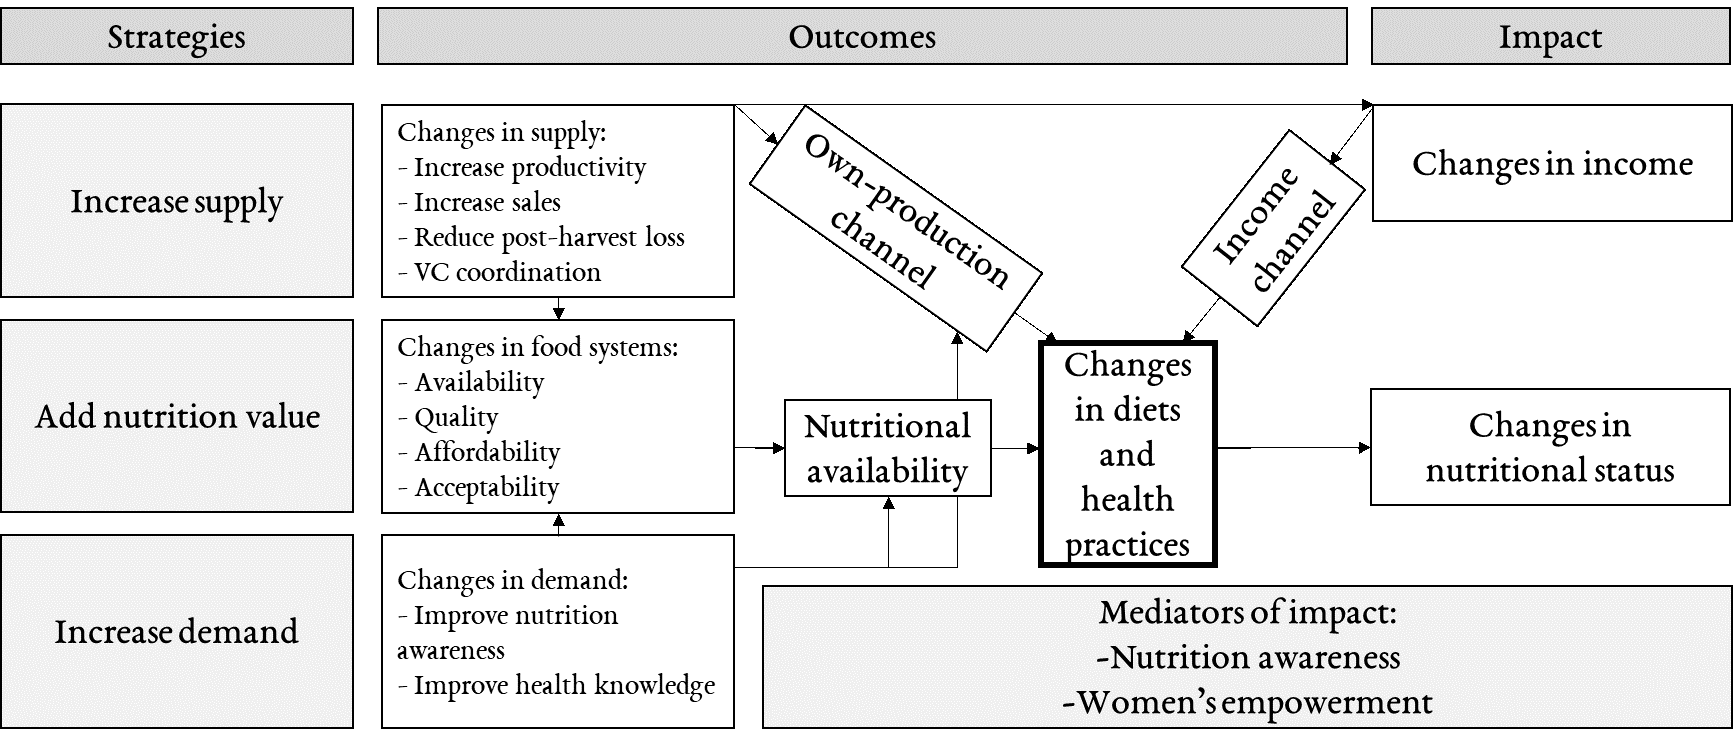
\includegraphics[width=1\textwidth]{figs_07/IFAD_frameworkv2.png}
  \captionsetup{singlelinecheck = off, justification=justified} %left justify caption
  \caption{Impact pathways of food system-based nutrition-specific and nutrition-sensitive interventions}
  \label{fig:01_1}
  %\small
  %\raggedright
  \vspace*{-3mm}
  \caption*{VC = value-chain \\
 	(Reproduced with permission from \citealp{DeLaPena2018})}

\end{figure}

\subsection{The prevalence and spatial distribution of food insecurity}
Our best estimates of chronic and hidden hunger globally are based on FBS. These estimates provide vital insights into the deficiencies of global and regional food supplies. FBS for energy are compiled annually -- providing insights into trends and macro level associations (such as conflict and climate change; \citealp{FAO2018}). Assessments of hidden hunger are less common (\citealp{Kumssa2015, Joy2014}). Estimates from FBS are limited by low-quality data, simplifying assumptions, under-representation of informal trade and subsistence food, and assumptions of equal access to food supplies (\citealp{Micha2018}). The accuracy of FBS has been assessed against nationally representative household microdata -- generally finding poor agreement, with some level of convergence (\citealp{Desiere2018, Gobbo2015, Dowler1985278}). The assumption that each individual in the population has equal access to food and utilises what they need, however, under-represents food insecurity and masks the spatial distribution of food insecurity (\citealp{Micha2018}).

In contrast to FBS, the household level assessments (24hR, FFQ and food (in)security proxies) can provide more accurate and spatially explicit prevalence estimates of food insecurity. The food insecurity experience scale (FIES), for example, has been implemented in 140 countries with samples of more than 1,000 respondents per country (\citealp{FAO2018}). However, as the FIES indicator only represents food insecurity of access, other aspects of food security such as diet diversity and nutrient adequacy do not have the same global scale and frequency of application. These knowledge gaps related to the prevalence and spatial distribution of food insecurity also have a bearing on our knowledge of the associations between food security and livelihoods.

\subsection{Associations between food security and rural livelihoods}
The research community has been exploring the associations between food insecurity and rural livelihoods on national and sub-national scales. The emerging areas of investigation have centred on the role that agricultural production (subsistence and market-orientated) and off-farm income plays in improving food insecurity of access, diet diversity and nutrient adequacy ratios. Income, and thus purchased foods has been found to be highly associated with dietary diversity in a majority of these studies, whereas food from subsistence production, while also significant, has had a limited association with dietary diversity (\citealp{Bellon2016, Koppmair2017325, Luckett20152479, Sibhatu201510657, Snapp2015, Dillon2014}). In comparison, \citet{Jones2016} and \citet{MKaibi2015} emphasised the positive relationship farm production has with nutrition metrics. In the most geographically diverse study to date, the role of farm production on nutrition was found to be of varying importance depending on market opportunities (\citealp{Sibhatu201510657}). These findings, however, are dependent on food security at the time of survey and, as mentioned previously, have a limited geographical scope -- limiting cross-site comparisons and more generalisable inference.

The limitations in performing cross-site comparisons are -- in part -- due to a lack of coordination between organisations. This lack of coordination has resulted in a ``multiplicity of survey instruments collecting information on various dimensions of food and nutrition security'' (\citealp[p.~30]{Carletto2013}). The impetus to harmonise rural household microdata comes as nationally representative studies have been constrained in uptake and frequency of implementation (\citealp{Desiere2018, Carletto2013}). Progress has been made to overcome this research gap over the past decade (e.g. \citealp{Carletto2009, Herrero2007}). A harmonised data collection effort, however, has still not yet been realised. \citet[p.39]{Carletto2013} suggest that this harmonisation can be developed over time, with a ``combination of short-term fixes and long-term methodological advancements''.


\subsection{Objectives}

The primary objective of this thesis was to characterise food and nutrition security in rural landholding households in predominantly mixed crop-livestock agricultural systems of sub-Saharan Africa (SSA). Characterisation in this respect refers to describing the multiple facets of food and nutrition security, and identifying their associations with livelihoods. The related hypothesis is that variation in livelihoods between communities are strongly influenced by agro-climatic conditions, market opportunities and productive assets. It is also hypothesised that nutrition-related outcomes to a certain extent are determined by the livelihood characteristics present in a community. Understanding the context-specific relationships between livelihoods and food security will be essential to inform nutrition-specific (e.g. supplementation \& fortification) and nutrition-sensitive interventions (e.g. agricultural interventions that indirectly improve nutrition).

The secondary objective was to improve the methodological basis of household level food security studies. The related hypotheses to this objective are: 1) existing rural household surveys can be improved upon based on critical evaluation of reliability and credibility, 2) the quantification of food and nutrition security can be integrated with rural household surveys to capture conditions throughout the year, independent of survey timing, 3) research efforts of multiple organisations can be harmonised by providing an effective tool (survey).


\section{Outline of the thesis}

This thesis proceeds by introducing the `rural household multi-indicator survey' -- RHOMIS. Chapter 2 provides a summary of the design principles, indicators and pilot applications of RHOMIS. The data quality associated with rural household surveys is then critically evaluated in Chapter 3. The results of Chapter 3 then have a bearing on the analysis and inference of the three proceeding observational chapters. Chapter 4 provides an assessment of the livelihoods and food security status of households in an urban linked, high potential region of Tanzania over a three-year period. Chapter 5 provides an assessment of the pathways to food security in northern Burkina Faso, with a specific focus on the consumption of home-produced food versus purchased food. Chapter 6 provides an assessment of dietary gaps across multiple locations in sub-Saharan Africa. Chapter 7 then provides a synthesis of findings in this thesis, drawing together common themes and identifying areas for future research. Figure 1.2 provides a diagrammatic overview of this thesis.

\begin{figure}
    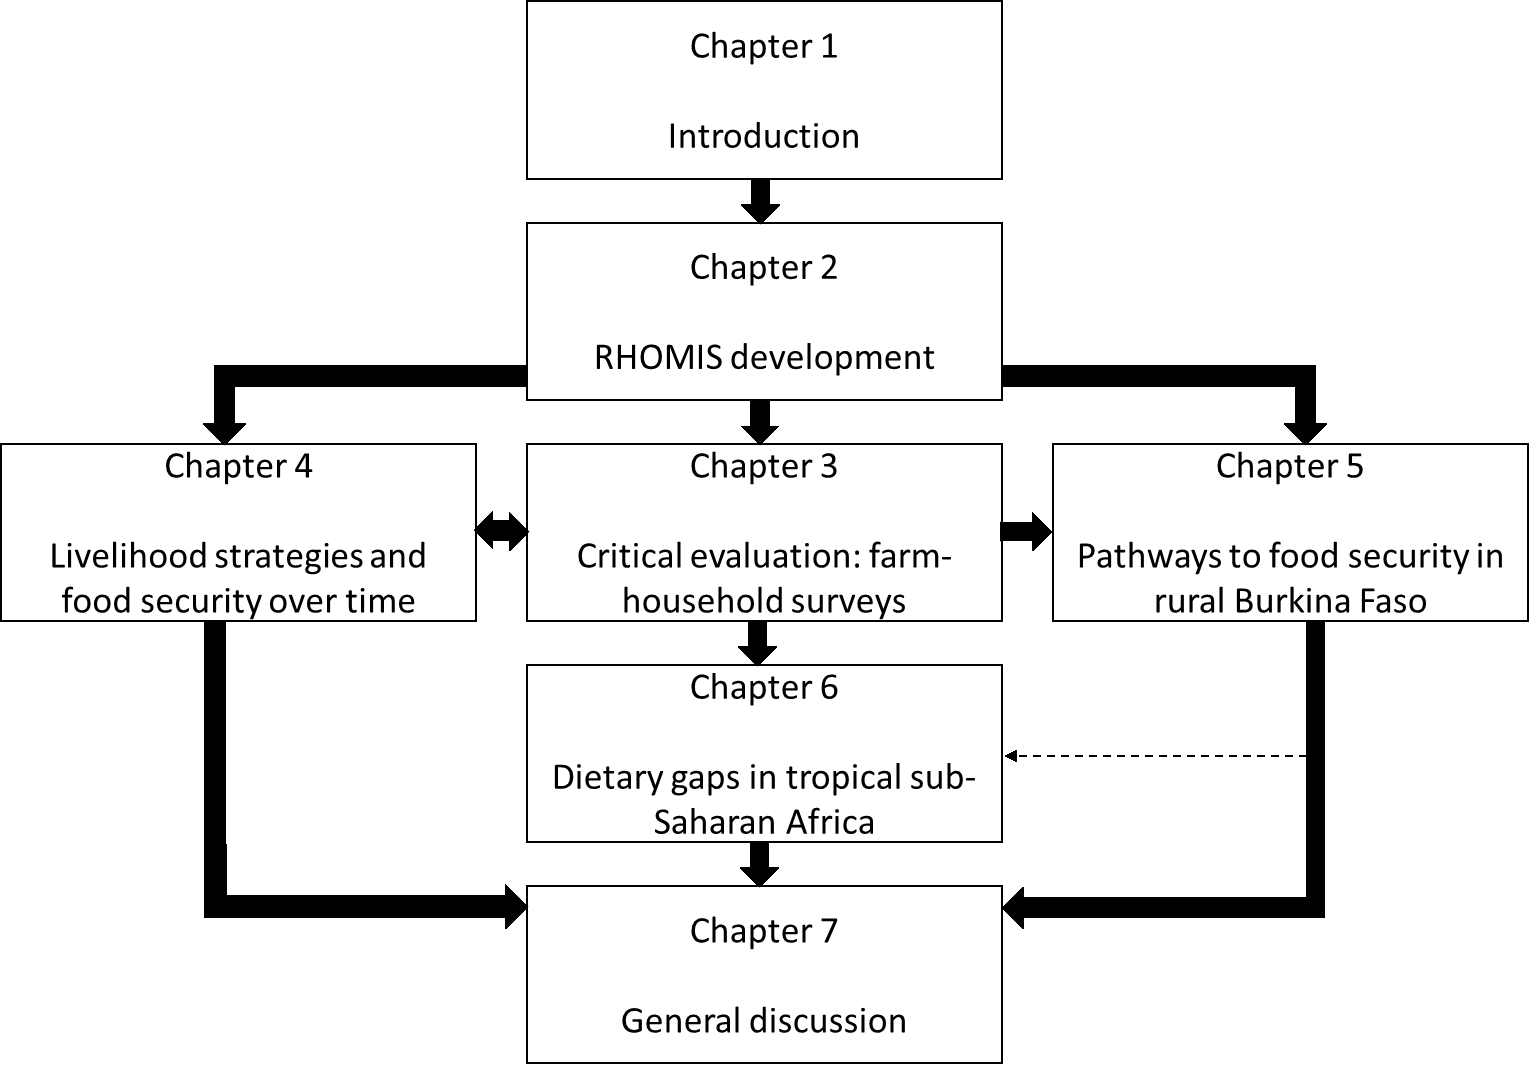
\includegraphics[width=0.8\textwidth]{figs_01/image1.png}

  \captionsetup{singlelinecheck = false, justification=raggedright} %left justify caption
  \label{fig:01_2}
  \caption{Overview of thesis structure}
\end{figure}

\subsubsection{Summary of study sites}

The primary objective of this research is addressed by drawing on harmonised rural household datasets across SSA. Research sites were located exclusively in rural communities and limited to landholding households. Sites were sampled from a diverse range of AEZs, with differing livelihoods and a presence of mixed crop-livestock systems. The study sites are presented in Figure \ref{fig:01_3}. Appendix Table \ref{tab:01_1} summarises the characteristics of study sites. A total of 9,126 households were sampled, of which, 4,323 households were located in warm semi-arid zones, 1,402 households were located in warm sub-humid and humid zones, 250 households were located in a cool semi-arid zone, 1,872 households were located in cool (sub)humid AEZs and two studies spanned multiple AEZs with 1,279 observations. Livestock keeping and staple crop cultivation were prominent livelihood activities in all sites (not represented in Appendix Table \ref{tab:01_1}). The presence of dairy, cash-crops and off-farm income opportunities differed by site. Market orientation and market access also differed. These harmonised rural household datasets were utilised in Chapters 2 to 6, with the majority of observations employed to explore dietary gaps in Chapter 6 (Appendix Table \ref{tab:01_1} summarises which chapter each site relates to).



\begin{figure}
  %\centering
    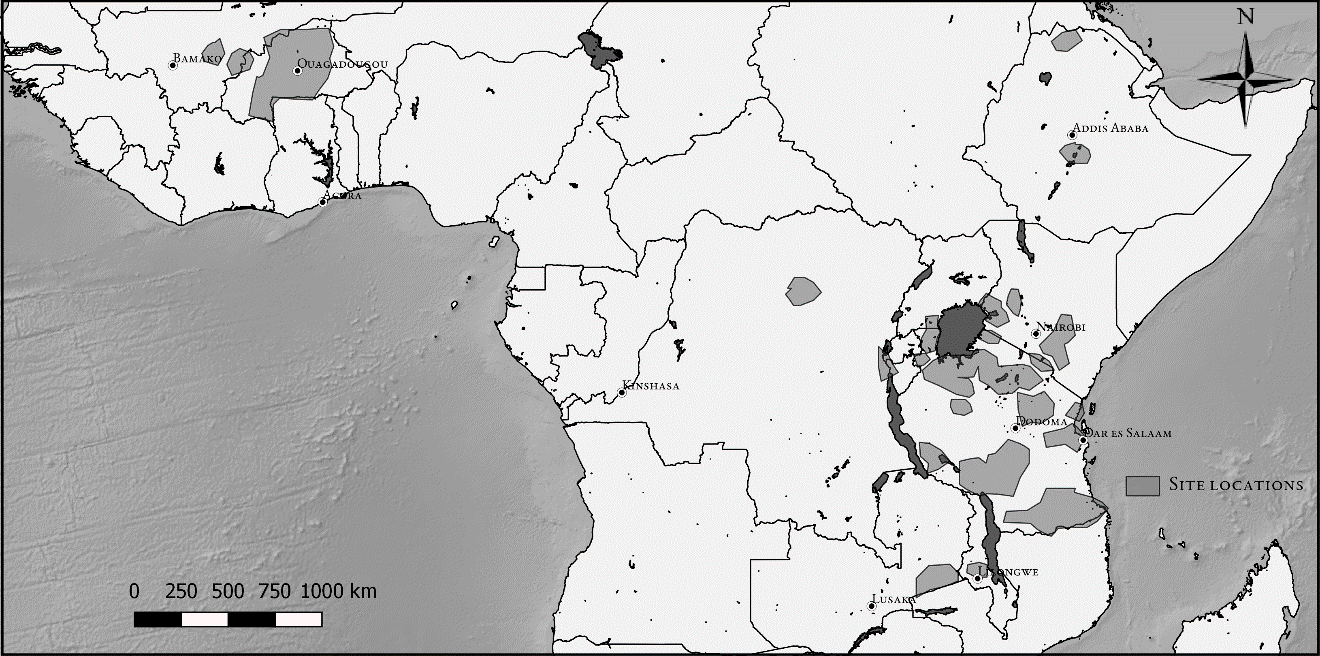
\includegraphics[width=1\textwidth]{figs_01/siteMap.png}
  \captionsetup{singlelinecheck = false, justification=justified} %left justify caption
  \caption{Map of study sites}
    \label{fig:01_3} %Label needs to come after caption
\end{figure}
